%%%%%%%%%%%%%%%%%%%%%%%%%%%%%%%%%%%%%%%%%%%%%%%%%%%
% PRESENTATION FOR SUMMER RESEARCH MEETING (2018)
% 
% Prithvi Thakur
% Geophysics research group
% Department of Earth and Environmental Science
% University of Michigan, Ann Arbor
%%%%%%%%%%%%%%%%%%%%%%%%%%%%%%%%%%%%%%%%%%%%%%%%%%%

\documentclass{beamer}

\mode<presentation>{
\usetheme{AnnArbor}
}

\usepackage{graphicx} % Allows including images
\usepackage{booktabs} % Allows the use of \toprule, \midrule and \bottomrule in tables

%------------------------------------------------
%           TITLE PAGE INFORMATION
%------------------------------------------------
\title[MFD in EQ Cycles]{Magnitude-Frequency Distribution of Simulated Earthquake Cycles in Damaged Fault Zones} 
\author{Prithvi Thakur}
\institute[UofM]
{
University of Michigan \\ % Your institution for the title page
\medskip
\textit{prith@umich.edu} % Your email address
}
\date{\today} % Date, can be changed to a custom date
%------------------------------------------------

%%%%%%%%%%%%%%%%
\begin{document}

% TITLE PAGE
\begin{frame}
    \titlepage 
\end{frame}

% TABLE OF CONTENTS
\begin{frame}
    \frametitle{Overview}
    \tabeleofcontents
\end{frame}

% MODEL DESCRIPTION
\section{Model Description}
\begin{frame}
    \frametitle{Model Description}
    \begin{figure}
        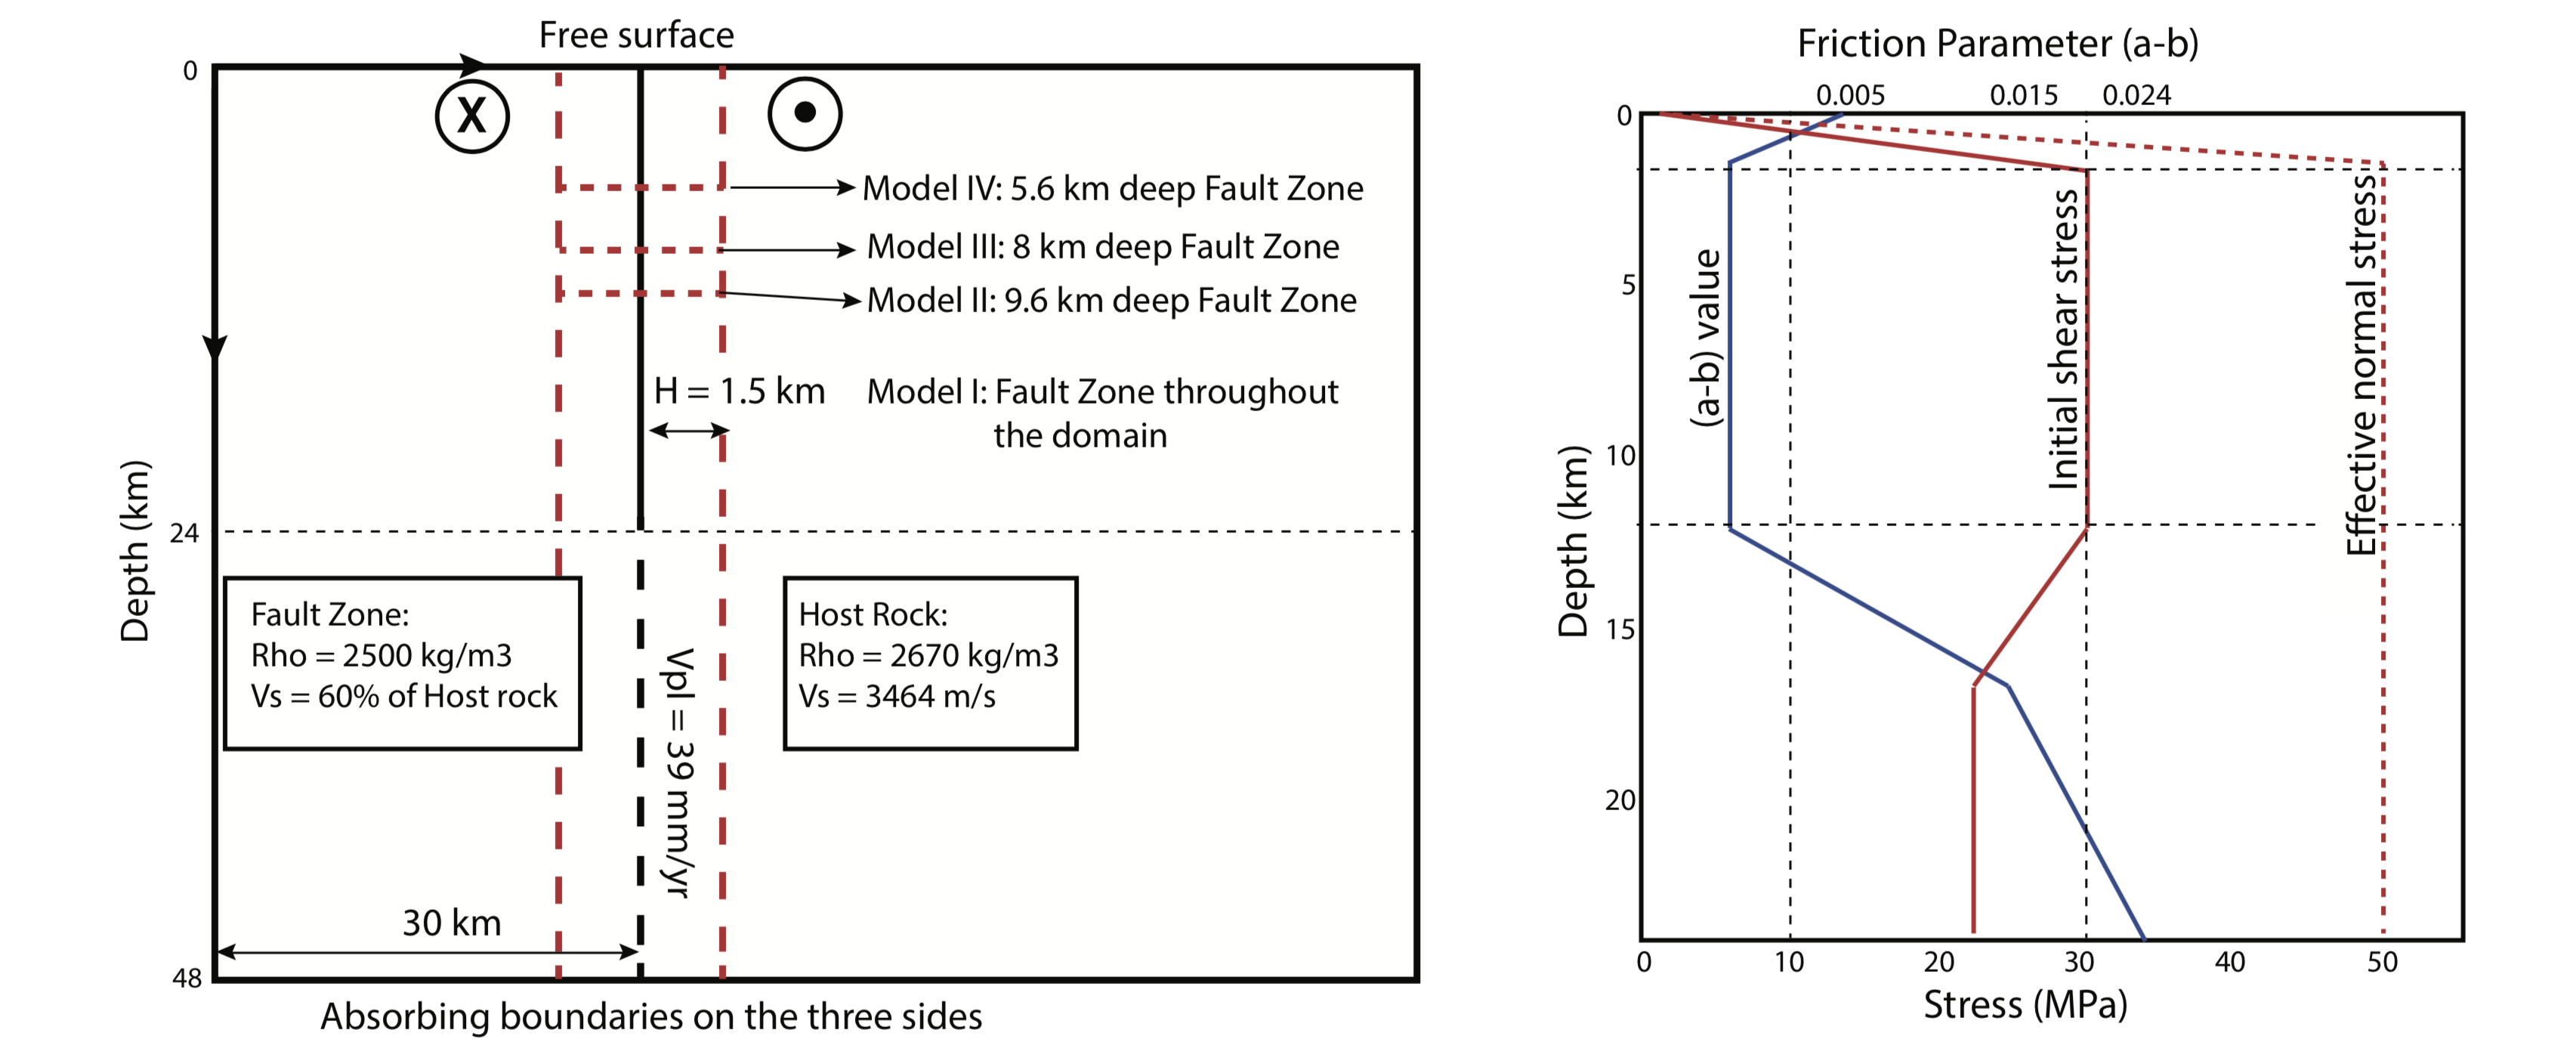
\includegraphics[width=0.9\linewidth]{images/model_setup}
    \end{figure}
\end{frame}

% OBSERVATIONS: PARKFIELD MFD PLOTS
\section{Natural Observations}
\begin{frame}
    \frametitle{Observations from San-Andreas Fault}
\end{frame}

% RESULTS PLOT
\section{Simulated Results}
\begin{frame}
    \frametitle{Simulated Magnitude-Frequency Distribution}
\end{frame}

% RESULTS PLOT
\section{Simulated Results}
\begin{frame}
    \frametitle{Simulated Magnitude-Frequency Distribution}
\end{frame}

% CONCLUSIONS
\section{Conclusions}
\begin{frame}
    \frametitle{Conclusions}
\end{frame}

% ENDING SLIDE
\begin{frame}
    \Huge{\centerline{That's All Folks!!}}
\end{frame}
\end{document} 
%%%%%%%%%%%%%%%%
